\documentclass[journal]{./IEEE/IEEEtran}
\usepackage{cite,graphicx}

\newcommand{\SPTITLE}{Automated Identification of Rice and Corn Pests(Order Hemiptera) through GLCM using K-Nearest Neighbors Algorithm}
\newcommand{\ADVISEE}{John Viscel M. Sangkal}
\newcommand{\ADVISER}{Concepcion L. Khan}

\newcommand{\BSCS}{Bachelor of Science in Computer Science}
\newcommand{\ICS}{Institute of Computer Science}
\newcommand{\UPLB}{University of the Philippines Los Ba\~{n}os}
\newcommand{\REMARK}{\thanks{Presented to the Faculty of the \ICS, \UPLB\
                             in partial fulfillment of the requirements
                             for the Degree of \BSCS}}
        
\markboth{CMSC 190 Special Problem, \ICS}{}
\title{\SPTITLE}
\author{\ADVISEE~and~\ADVISER%
\REMARK
}
\pubid{\copyright~2014~ICS \UPLB}

%%%%%%%%%%%%%%%%%%%%%%%%%%%%%%%%%%%%%%%%%%%%%%%%%%%%%%%%%%%%%%%%%%%%%%%%%%

\begin{document}

% TITLE
\maketitle

% INTRODUCTION
\section{Introduction}

\subsection{Background of the Study}
Philippines is an agricultural country. Environmental conditions such as soil and weather conditions make the Philippines suitable for planting crops as a source of living. Rice and Corn are two of the most important and primary source of food in the country, however these crops may lose its quantity and quality when attacked by different pests. Farmers lose an estimated average of 37\% of their rice crop to pests and diseases every year. Therefore it is top priority to find an effective method to control the damage of the pests.In addition to good crop management, timely and accurate diagnosis can significantly reduce losses.\cite{electronic_irri}

\subsection{Statement of the Problem}
One vital issue with field crop is identification of pests. When symptoms of any pests take place on crops in fields, proper action should be taken to control it in order to minimize loss to farmers. Farmers use their experience or knowledge and reference guide books for the correct action to take place. If they do not have proper knowledge, then misidentification of any pests can take place and incorrect control measures like non-affecting pesticides may be used leading to waste of effort, time, and money and it may also lead to serious problems to crops
	
Farmers may also approach any agricultural experts to advise them regarding detection and identification of pests affecting their crops and how to manage them. However, Sometimes, they have to go long distances to consult an expert and may find themselves wasting their time and effort because the expert may not be available at the time. Also, the expert the farmer consults may not be in a position to advise.
	
In order to avoid wasting resources and to produce maximum yield of crops, an online library and system for identifying possible pests through analysis of pest images needs to be designed for farmers to easily identify pests.\cite{article_kandalkar2}


\subsection{Significance of the Study}
Enormous agricultural yield is lost every year, due to rapid infestation by pests and insects thus plant pest identification is important for food security, quality of life and a stable agricultural economy. If farmers properly identify these pests then they can take preventive as well as control measures such as spraying pesticides to increase production.\cite{article_kandalkar3} By developing an online library and application that extracts observable features of a pest from an image through digital image processing techniques and classify the species of the pest, farmers who have few experience and knowledge about pest will have an initial diagnosis of the pest that infected the crops. 


\subsection{Objectives}
Generally, this study aims to devise an online library system of pest and diseases for crops integrated with a system that will identify the possible species of the pest under the order Hemiptera in a pest image through digital image processing and provide all relevant information about the possible species of the pests. Specifically, it aims to:
\pubidadjcol
	\begin{itemize}
	\item Develop a pests and diseases library for rice and corn
	\item Extract texture features such as energy, entropy, homogeneity, and correlation using GLCM
    \item Identify the possible pest species through analysis of extracted features
	\item Provide relevant information about the possible species of the pest  such as destructive stage, plant part and growth stage damaged, nature of damage, management practices and environmental factors
	\item Find the percentage of the accuracy of the system
	\end{itemize}

\subsection{Scope and Limitations}
The library of pests only consists of major pests and diseases for rice and corn.

This study only identifies pest under the order Hemiptera(True Bugs). The features of the pest that will be used to identify the species of the pest are texture features such as energy, entropy, homogeneity, and correlation which will be extracted using GLCM matrix.

The users of the system is assumed to capture the pest image using smart phone camera or digital camera.

% REVIEW OF RELATED LITERATURE
\section{Review of Related Literature}

\subsection{Pest Order Hemiptera}
		Order Hemiptera are characterized by 2 pairs of wings, although some species may be wingless and others have only forewings. Wings are generally membranous but in some species the forewings may be hardened at the base. They also have piercing or sucking mouthparts appearing as a sharply pointed tube known as a proboscis or rostrum, which extends from the underside of the head. Their eyes may be compound of various forms. Hemipterans' antennae vary and may be either short, or long and conspicuous. The young of hemipterans look like small adults. Some bugs may be mistaken for beetles but can be distinguished by their mouthparts as beetles have mandibulate mouthparts while bugs have sucking/piercing mouthparts.

		This order is divided into 3 suborders; true bugs (Heteroptera); hoppers (Auchenorrhyncha) and; aphids, scale insects, lerps and mealy bugs (Sternorrhyncha).

		Figure 1 shows the general life cycle of Hemipterans. Hemipterans develop by incomplete metamorphosis and young (or nymphs) generally resemble small, wingless adults in general structure although their colour and markings may be very different. In some species such as cicadas, the nymphs who are specialised for burrowing appear quite different from the adults. Nymphs will moult 6 to 8 times depending on the species before they attain maturity.

				\begin{figure}[h!]
			  		\centering
					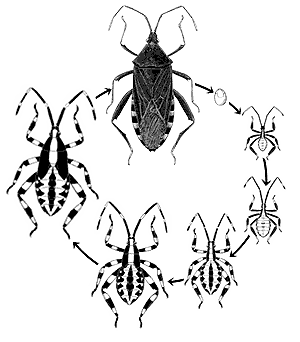
\includegraphics[scale=0.5]{images/bug_life_cycle.png}
					\caption{Life Cycle of Order Hemiptera}
				\end{figure}

		Most species of Hemiptera are plant feeders, sucking sap with many causing considerable damage to crops, ornamental garden plants such as roses, shrubs and trees. Some species are bloodsuckers of mammals and birds while others are predators that feed on other invertebrates, including some pest species and are therefore beneficial to man.

		The proboscis of hemipterans contains cutting blades and a two-channelled tube. Hemipterans feed by cutting into a plant or animal and sending saliva down one of the tubes to begin digestion. The liquid food is then sucked up the other tube.\cite{electronic_bugs}

\subsection{Some Online Pest Library and Their Features}
	\begin{enumerate}
	\item Orkin.com\\
	-Orkin.com is a commercial website which provides a library of pests not only found in field crops but also in the house and in the wild. It implements a system for the user to schedule or contact with a specialist. It also has a search engine for pests and displays vital informations about them such as common name of pest, scientific name, facts, identification, control, appearance, behavior, diet, and habits.\cite{electronic_orkin}\\
	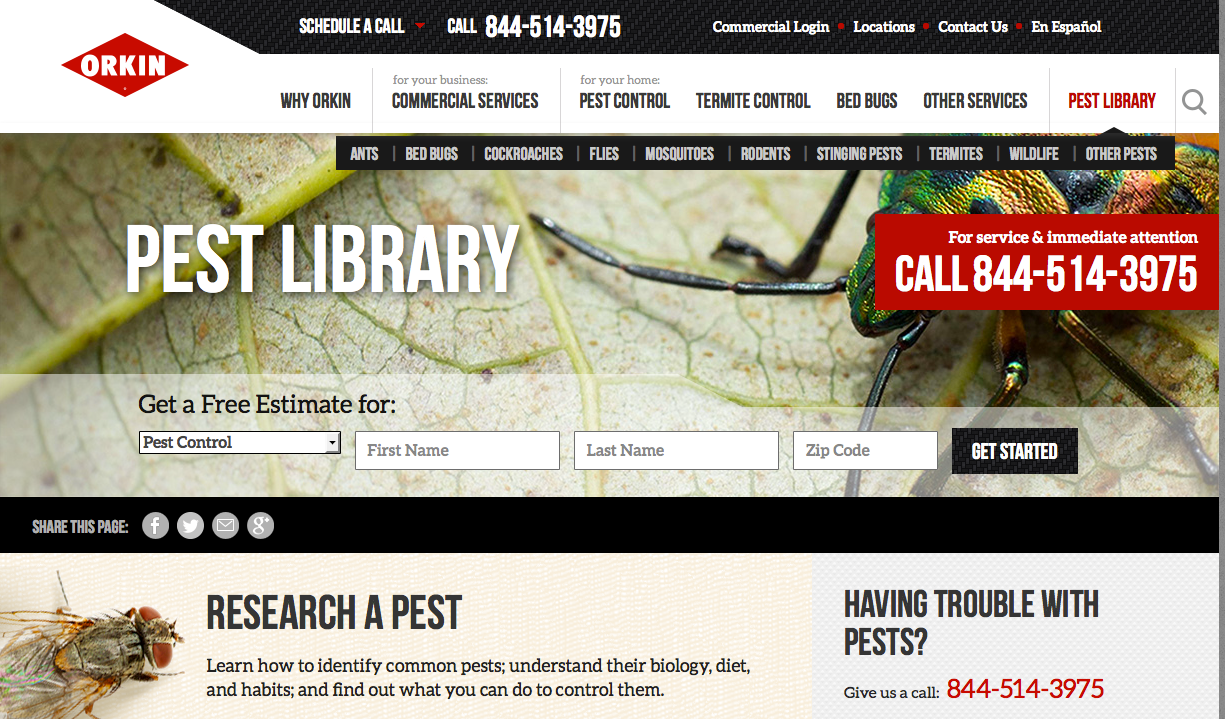
\includegraphics[scale=0.17]{images/orkin.png}	\\
	\item IRRI Rice Knowledge Bank\\
	-IRRI's Rice Knowledg Bank provides a detailed step-by-step control and prevention of pest to limit the damage as well as a library of pests that provides information like common name of pest, scientific name, what it does, why and where it occurs, how to identify, why is it important, and how to manage it.\cite{electronic_irri}\\
	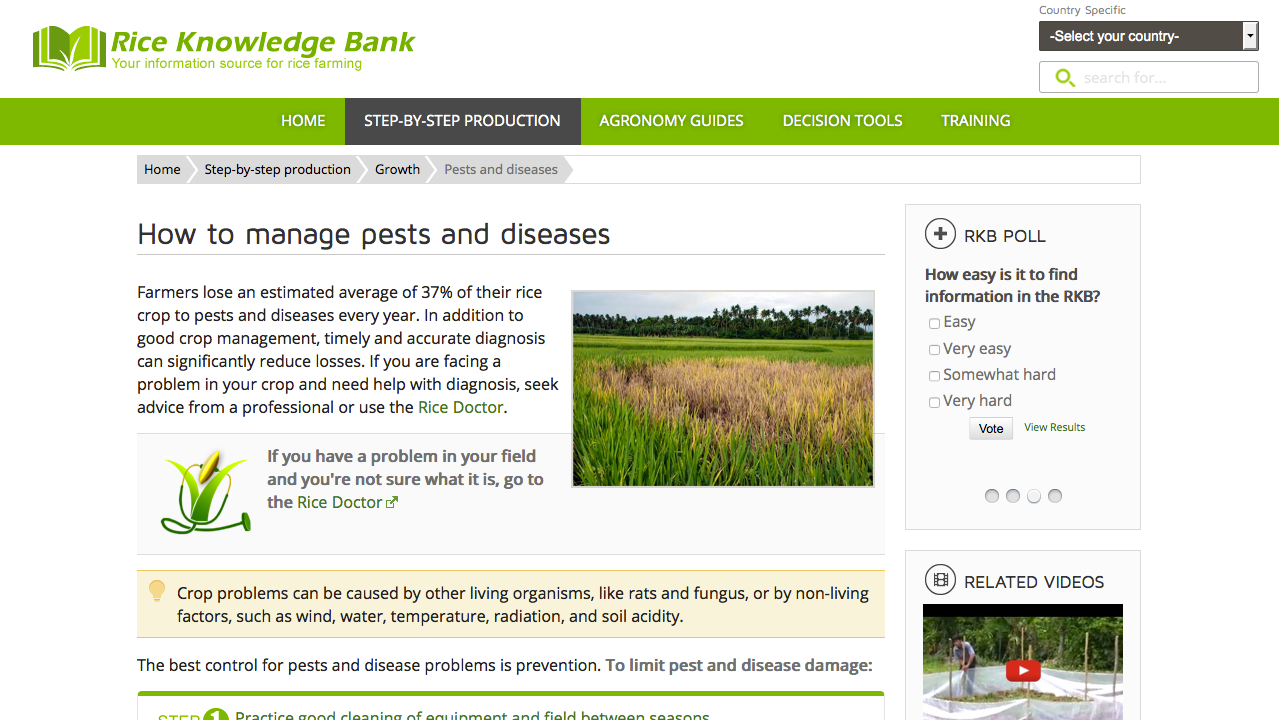
\includegraphics[scale=0.17]{images/irri.png}	\\
	\end{enumerate}

\subsection{Image Processing for Pest Species Identification}
There have been many recent studies around the world about pest identification and detection through image processing. In 2014, \cite{article_kandalkar} developed a decision support system that uses image segmentation to extract the pest from the image then extract the features of the pest such as color and shape. The features will be saved in a databased with the name of the pest. A Support Vector Machine classifier would be finding out the type of pest then the system will give preventive and control measures to the user.

In 2013, \cite{article_mundada} used the same method as Kandalkar and Deorankar but the features they extracted are entropy, mean, standard deviation, contrast, energy, correlation, and eccentricity.

In 2010, \cite{conf_zhu} developed a novel method to classify insects by analyzing color histogram and GLCM (Gray-Level Co-occurrence Matrices) of wing images is proposed. The image is preprocessed to get the ROI(Region of Interest) then the color space is converted to HSI (Hue-Saturation-Intensity). Color histograms of the ROI are generated from hue and saturation distributions. Afterward, the color image is converted to grayscale and their GLCM(Gray Level Co-occurence Matrices) features are extracted. K-Nearest Neighbor algorithm is used for classification. A lepidopteran insect database with 100 species is used to test the method. With a recognition rate of 71.1\% and an ideal time performance achieved, the experimental results testify the efficiency of proposed method.

\cite{article_zhang} made an automatic identification system of agricultural pest based on machine vision. They extracted 12 features including color, area, perimeter, fractal dimension, and ridgelet edge moment. They implemented feature selection to select 7 features out of the 12. Afterwards, Back Propagation neural network classifier was used to identify the pests. The pest recognition rate for 8 species was 85.7\% which shows that the system is efficient.

In 2011, \cite{article_alsaqer} used template matching to recognize pecan weevils. Five recognition methods were implemented: Normalize cross-correlation, Fourier Descriptors, Zernike moments, String matching, and Regional properties. They collected 205 pecan weevils for the training set and randomly selected 30 pecan weevils and 74 other insects for the testing set. The results showed that Region-based methods were better in representing and recognizing biological objects such as pests. The optimum result among the tested order of Zernike moments was found to be at the order 3. When the Zernike moments and Region properties recognition methods were used in combination, it achieved a recognition rate of 100\% and a processing time of 0.44 sec which proves the efficiency of the method.

\cite{article_cho} conducted a study for automatic identification of whiteflies, aphids, and thrips. The size and color components of the object were selected as features for identification because aphids have small variation in color information and the body size is substantially different from other species. The identification error for whiteflies and thrips was reduced when the data for aphids was analyzed first.

In 2013, \cite{article_fina} used k-means clustering algorithm and correspondence filters to automatically detect and recognize pest from an image. The detected the data set by partitioning the data space into Voronoi cells in order to find clusters of comparable spatial extents. With this, they separated the pest from the background. By extracting variant distinctive attributes between the pest and its habitat and using correspondence filters, they identified the plant pest and obtained correlation peak values for different datasets. The study showed that the recognition probability from the pest image is directly proportional to the height of the output signal and inversely proportional to the viewing angles. The correspondence filter can achieve rotational invariance of pests up to angles of 360 degrees which proves the effectiveness of the algorithm.

In 2014, \cite{article_kandalkar3} proposed a new approach. Saliency map based segmentation was used to separate the foreground from the background. Afterwards, features were extracted from the segmented image of the pest. One feature is energy which is computed via discrete wavelet transform. The features later on was stored with the database along with the name of the pest. With back propagation neural network, the pest is classified and control and preventive measures were provided.

The preceeding review shows that there have been many methods and algorithms developed for automated pest identification and each has its own advantage and disadvantages. There has been no study on the method to automatically identify pest under order Hemiptera making this study relevant.

% MATERIALS AND METHODS
\section{Materials and Methods}

\subsection{Materials}
Data for this study will be actual images of pests(Hemiptera) taken from IRRI and other fields. A digital camera and smart phone will be used to collect images. Images will be taken under daylight with no flash.

\subsection{Development Tools}
	The system will be developed under Ubuntu Operating System. To be able to implement the system, it will be necessary to install and use the following:
	\begin{enumerate}
		\item Content Management System(CMS): A Content Management System allows publishing, editing and modifying content, organizing, deleting as well as maintenance from a central interface. It will be easier for non-developers to maintain a system. WordPress 4.0 shall be used for the pest and diseases library where the identification of pest will be integrated. WordPress is built on PHP and MySQL.\cite{electronic_wp}
		\item Digital Image Processing Library: OpenCV is an open source library for image processing. It is optimized in C++ but it also has Python and Java Interfaces. For this development, the C++ Interface will be used. It will be integrated with WordPress.\cite{electronic_opencv}
		\item Database: MySQL 5.1.41 will be used as database for this application. It is an open-source database management system. This is where the information about the different pests and diseases shall be stored and the data for the pest and diseases identification.
	\end{enumerate} 

\subsection{System Implementation}
	The system consists of a pests and diseases library for crops where the system for pest identification will be integrated to. Figure 2 shows the phases undergone by each pest image. It is composed of five basic phases of digital image processing. The first phase isthe collection of pest images of order Hemiptera in order to create a database. Using saliency map techniques, the image is segmented to separate the pest from the background. Features of the segmented image like energy of an image is extracted and these features are stored in the database with the name of the pest. Using K-nearest neighbors algorithm, the pest will be identified and the system will give relevant information to control it.\\
	\begin{figure}[h!]
  		\centering
		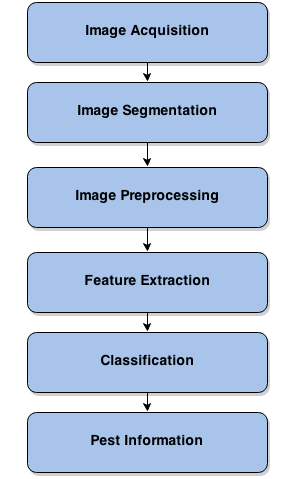
\includegraphics[scale=0.5]{images/flowchart.png}
		\caption{Methodology Phases}
	\end{figure}

	\subsubsection{Image Acquisition}
	Images for the training and input data will be obtained using a digital camera or a scanner and will be uploaded to the system. For this study, a database of the features from the training data will be needed for classifying the pest to its proper species.
	\subsubsection{Image Segmentation}
	Image Segmentation is the process of partitioning an image into homogenous groups. Its goal is to cluster pixels into noticeable image regions.\cite{electronic_segmentation} For this study, adaptive thresholding will be implemented to segment the image. Using segmentation, the pest image, which is the foreground will be extracted and will be given to the image preprocessing stage.
	\subsubsection{Image Preprocessing}
	Image Preprocessing involves removing unwanted distortions, degradation, and noise during the image segmentation.\cite{electronic_preprocessing} Processes such as median filter, binary erosion, and binary dilation will be used to restore the pest image as close as possible to its original state. This process outputs a corrected image of the pest then it will be passed to the feature extraction phase.
	\subsubsection{Feature Extraction}
	A feature can be also viewed as a \"point of interest\" for image description. Properties of a good feature include consistency over several images of the same scene, invariant towards certain transformations, insensitive to noise, and salient or noticeable. A feature should be some quantifiable property of an object such that it quantifies significant characteristics of the object. Image features usually include color, shape and texture features.\cite{electronic_feature} 

	In this study, a gray-level co-occurrence matrix(GLCM) will be generated and normalized to compute the texture features. A gray-level co-occurrence matrix(GLCM) is esentially a two-dimensional histogram in which the \textit{(i,j)th} element is the frequency of event \textit{i} co-occurs with event \textit{j}. A co-occurrence matrix is specified by the relative frequencies P(i,j,d,$ \phi $) in which two pixels, separated by distance \textit{d}, occur in a direction specified by the angle $ \phi $, one with gray level \textit{i} and the other with gray level \textit{j}. A co-occurrence matrix is therefore a function of distance \textit{d}, angle $ \phi $ and grayscales \textit{i} and \textit{j}.\cite{article_manaa} 

	For this study, the features to be computed from the GLCM for classifying the pest are Entropy, Homogeneity, Energy, and Correlation.
		\begin{enumerate}
		\item Entropy in any system represents disorder, where in the case of texture analysis is a measure of its spatial disorder.\\
				\begin{figure}[h!]
			  		\centering
					\includegraphics[scale=0.5}{images/entropy.png}
				\end{figure}

		\item Homogeneity measures the uniformity of the non-zero entries in the GLCM.\\
				\begin{figure}[h!]
			  		\centering
					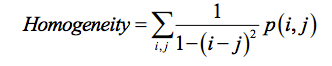
\includegraphics[scale=0.5]{images/homogeneity.png}
				\end{figure}

		\item Energy is a measure of local homogeneity and therefore it represents the opposite of the Entropy. Basically this feature will tell us how uniform the texture is.\\
				\begin{figure}[h!]
			  		\centering
					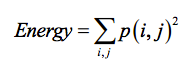
\includegraphics[scale=0.5]{images/energy.png}
				\end{figure}

		\item The Correlation texture measures the linear dependency of gray levels on those of neighboring pixels.\\
				\begin{figure}[h!]
			  		\centering
					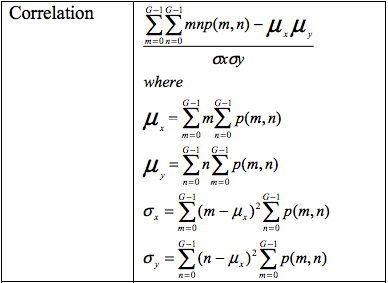
\includegraphics[scale=0.5]{images/correlation.png}
				\end{figure}
		\end{enumerate}
	The features that will be extracted will be the input for the classification stage.
	%explain features
	\subsubsection{Classification}
	With the help of K-nearest neighbors algorithm, the possible species and life stage of the pest will be identified and the system will give preventive as well as control measures to it.

	K-nearest neighbors algorithm is a \"non parametric lazy learning algorithm\". It means that it does not make any assumptions on the underlying data distribution. It is a lazy learning algorithm because it defers the decision to generalize beyond the training examples until a new query is encountered. stores all training samples and predicts the response by analyzing a certain number (K) of the nearest neighbors of the sample.\cite{electronic_knn} 

	Training samples are vectors in a multidimensional feature space, each with a class label. In the training phase, the feature vectors and class labels of the training samples will be stored in a database.

	For the classification phase, a number \textit{k} will be defined by the programmer. The unlabeled vector(a query) is classified by assigning the label which is the most frequent among the \textit{k} training samples nearest to that query point.

	To find the input data's K nearest neighbors in this study, Euclidean Distance will be used to calculate the distance.

% BIBLIOGRAPHY
\bibliographystyle{./IEEE/IEEEtran}
\bibliography{./cs190-ieee}
% \nocite{*}

\end{document}
 
